%
\documentclass[12pt,journal,compsoc]{IEEEtran}
% The Computer Society requires 12pt.
% If IEEEtran.cls has not been installed into the LaTeX system files,
% manually specify the path to it like:
% \documentclass[10pt,journal,compsoc]{../sty/IEEEtran}


% For Computer Society journals, IEEEtran defaults to the use of 
% Palatino/Palladio as is done in IEEE Computer Society journals.
% To go back to Times Roman, you can use this code:
%\renewcommand{\rmdefault}{ptm}\selectfont





% Some very useful LaTeX packages include:
% (uncomment the ones you want to load)



% *** MISC UTILITY PACKAGES ***
%
%\usepackage{ifpdf}
% Heiko Oberdiek's ifpdf.sty is very useful if you need conditional
% compilation based on whether the output is pdf or dvi.
% usage:
% \ifpdf
%   % pdf code
% \else
%   % dvi code
% \fi
% The latest version of ifpdf.sty can be obtained from:
% http://www.ctan.org/tex-archive/macros/latex/contrib/oberdiek/
% Also, note that IEEEtran.cls V1.7 and later provides a builtin
% \ifCLASSINFOpdf conditional that works the same way.
% When switching from latex to pdflatex and vice-versa, the compiler may
% have to be run twice to clear warning/error messages.






% *** CITATION PACKAGES ***
%
\ifCLASSOPTIONcompsoc
  % IEEE Computer Society needs nocompress option
  % requires cite.sty v4.0 or later (November 2003)
   \usepackage[nocompress]{cite}
   \usepackage{citesort}
\else
  % normal IEEE
  % \usepackage{cite}
\fi
% cite.sty was written by Donald Arseneau
% V1.6 and later of IEEEtran pre-defines the format of the cite.sty package
% \cite{} output to follow that of IEEE. Loading the cite package will
% result in citation numbers being automatically sorted and properly
% "compressed/ranged". e.g., [1], [9], [2], [7], [5], [6] without using
% cite.sty will become [1], [2], [5]--[7], [9] using cite.sty. cite.sty's
% \cite will automatically add leading space, if needed. Use cite.sty's
% noadjust option (cite.sty V3.8 and later) if you want to turn this off.
% cite.sty is already installed on most LaTeX systems. Be sure and use
% version 4.0 (2003-05-27) and later if using hyperref.sty. cite.sty does
% not currently provide for hyperlinked citations.
% The latest version can be obtained at:
% http://www.ctan.org/tex-archive/macros/latex/contrib/cite/
% The documentation is contained in the cite.sty file itself.
%
% Note that some packages require special options to format as the Computer
% Society requires. In particular, Computer Society  papers do not use
% compressed citation ranges as is done in typical IEEE papers
% (e.g., [1]-[4]). Instead, they list every citation separately in order
% (e.g., [1], [2], [3], [4]). To get the latter we need to load the cite
% package with the nocompress option which is supported by cite.sty v4.0
% and later. Note also the use of a CLASSOPTION conditional provided by
% IEEEtran.cls V1.7 and later.





% *** GRAPHICS RELATED PACKAGES ***
%
\ifCLASSINFOpdf
   \usepackage[pdftex]{graphicx}
  % declare the path(s) where your graphic files are
  % \graphicspath{{../pdf/}{../jpeg/}}
  % and their extensions so you won't have to specify these with
  % every instance of \includegraphics
  % \DeclareGraphicsExtensions{.pdf,.jpeg,.png}
\else
  % or other class option (dvipsone, dvipdf, if not using dvips). graphicx
  % will default to the driver specified in the system graphics.cfg if no
  % driver is specified.
  % \usepackage[dvips]{graphicx}
  % declare the path(s) where your graphic files are
  % \graphicspath{{../eps/}}
  % and their extensions so you won't have to specify these with
  % every instance of \includegraphics
  % \DeclareGraphicsExtensions{.eps}
\fi
% graphicx was written by David Carlisle and Sebastian Rahtz. It is
% required if you want graphics, photos, etc. graphicx.sty is already
% installed on most LaTeX systems. The latest version and documentation can
% be obtained at: 
% http://www.ctan.org/tex-archive/macros/latex/required/graphics/
% Another good source of documentation is "Using Imported Graphics in
% LaTeX2e" by Keith Reckdahl which can be found as epslatex.ps or
% epslatex.pdf at: http://www.ctan.org/tex-archive/info/
%
% latex, and pdflatex in dvi mode, support graphics in encapsulated
% postscript (.eps) format. pdflatex in pdf mode supports graphics
% in .pdf, .jpeg, .png and .mps (metapost) formats. Users should ensure
% that all non-photo figures use a vector format (.eps, .pdf, .mps) and
% not a bitmapped formats (.jpeg, .png). IEEE frowns on bitmapped formats
% which can result in "jaggedy"/blurry rendering of lines and letters as
% well as large increases in file sizes.
%
% You can find documentation about the pdfTeX application at:
% http://www.tug.org/applications/pdftex



%\usepackage{ps4pdf}
% dvi->ps workflow is required to use such packages as psfrag.sty and
% pstricks.sty. However, Rolf Niepraschk's ps4pdf.sty provides a way to
% apply psfrag/pstricks effects to .eps figures and then get the resultant
% figures in .pdf form. Thus, providing an easier way for migrating from
% .eps to .pdf figures. After ps4pdf.sty loads, if:
% 1. producing .dvi output: the output file will consist ONLY of the
%    figures (or other constructs encased within \PSforPDF commands)
% 2. producing .pdf output: pdflatex will look in the filename-pics.pdf
%    file, where filename is the basename of the tex document, for the
%    graphics (or other constructs encased within \PSforPDF commands).
%    NOTE: If you ever change your figures, you must remember to remake
%    the filename-pics.pdf file.
%
% This way you can do a:
% 
% latex filename
% dvips -Ppdf -o filename-pics.ps filename.dvi
% ps2pdf filename-pics.ps filename-pics.pdf
% 
% to produce a filename-pics.pdf graphics container that contains
% .pdf versions of the graphics with psfrag, pstricks, etc. features.
% Note that you will not typically be able to view the figures in 
% filename-pics.ps because of an offset. However, you will be able to
% view them in filename-pics.pdf. Also, note that when ps4pdf is in effect
% with .dvi output, you may get harmless over/under full box warnings - 
% ignore them. 
% Then, run pdflatex:
% 
% pdflatex filename
% 
% to use pdflatex to make PDF output, automatically using the figures in
% filename-pics.pdf. Alternatively, you could use dvips -i option to
% obtain separate .pdf files for each figure:
%
% dvips -Ppdf -i -E -o fig filename
%
% then convert each figure to pdf via a command such as epstopdf and then
% use pdflatex with these pdf figures and then to dispense with ps4pdf.
%
% Remember to rerun through latex/dvips/ps2pdf if you ever change your
% figures so that filename-pics.pdf gets updated.
% ps4pdf requires David Kastrup's preview-latex and a recent LaTeX system
% (circa 2001 or later). The ps4pdf package and documentation can be
% obtained at: http://www.ctan.org/tex-archive/macros/latex/contrib/ps4pdf/
% The preview-latex package and documentation can be obtained at:
% http://www.ctan.org/tex-archive/macros/latex/contrib/preview/
%
% provide a bogus \PSforPDF, even when not loading pd4pdf. This way we can
% stop loading ps4pdf.sty if we choose to make separate .pdf versions of
% each of our figures.
\providecommand{\PSforPDF}[1]{#1}
% Note that in order for ps4pdf to work, all commands related to psfrag,
% pstricks, etc. must be called within the PSforPDF command. This applies
% even when *loading* via \usepackage psfrag.sty, etc.


%\PSforPDF{\usepackage{psfrag}}
% psfrag.sty was written by Craig Barratt, Michael C. Grant, and
% David Carlisle. It allows you to substitute LaTeX commands for text in
% imported EPS graphic files. In this way, LaTeX symbols can be placed into
% graphics that have been generated by other applications. You must use
% latex->dvips->ps2pdf workflow (not direct pdf output from pdflatex) if
% you wish to use this capability because it works via some PostScript
% tricks. Alternatively, the graphics could be processed as separate files
% via psfrag and dvips, then converted to PDF for inclusion in the main file
% which uses pdflatex. ps4pdf.sty (above) provides a way of doing this all
% at once within the main file.
% Docs are in "The PSfrag System" by Michael C. Grant and David Carlisle.
% There is also some information about using psfrag in "Using Imported
% Graphics in LaTeX2e" by Keith Reckdahl which documents the graphicx
% package (see above). The psfrag package and documentation can be obtained
% at: http://www.ctan.org/tex-archive/macros/latex/contrib/psfrag/
% 
% Note that the current version of psfrag does not "turn itself off" when
% running under pdf output. This will result in a harmless warning
% about a non-PDF \special. However, to silence this, a bogus psfrag
% command can be provided instead of loading psfrag.sty when PDF output
% is being used. Thus, a more complex alternative conditional loading scheme
% can be employed instead of the straightforword way above:
%
%\ifCLASSINFOpdf
% if outputting PDF, do not use or load psfrag.sty as current versions
% output a non-PDF special that generates a harmless, but annoying warning.
% Instead, we provide a bogus \psfrag command that does nothing with
% its arguments. This is a tad tricky because \psfrag can have up to six
% arguments four of which are optional: \psfrag{}[][][][]{}
% Code based on that in psfrag.sty
%\makeatletter
%\def\psfrag{\@ifstar{\@BOGUSpsfraga}{\@BOGUSpsfraga}}
%\def\@BOGUSpsfraga{\begingroup
%   \@makeother\"\@makeother\*\@makeother\!\@makeother\~%
%   \@makeother\:\@makeother\\\@makeother\%\@makeother\#%
%   \@makeother\ \@BOGUSpsfragb}
%\def\@BOGUSpsfragb#1{\endgroup
%                \@ifnextchar [{\@BOGUSpsfragc}%
%                              {\@BOGUSpsfrag}}
%\def\@BOGUSpsfragc[#1]{\@ifnextchar [{\@BOGUSpsfragd}%
%                                     {\@BOGUSpsfrag}}
%\def\@BOGUSpsfragd[#1]{\@ifnextchar [{\@BOGUSpsfrage}%
%                                     {\@BOGUSpsfrag}}
%\def\@BOGUSpsfrage[#1]{\@ifnextchar [{\@BOGUSpsfragf}%
%                                     {\@BOGUSpsfrag}}
%\def\@BOGUSpsfragf[#1]{\@BOGUSpsfrag}
%\def\@BOGUSpsfrag#1{\ignorespaces}
%\makeatother
%\else
% using dvi output, load psfrag, but funnel it through PSforPDF
% as required by ps4pdf.sty
%\PSforPDF{\usepackage{psfrag}}
%\fi





% *** MATH PACKAGES ***
%
%\usepackage[cmex10]{amsmath}
% A popular package from the American Mathematical Society that provides
% many useful and powerful commands for dealing with mathematics. If using
% it, be sure to load this package with the cmex10 option to ensure that
% only type 1 fonts will utilized at all point sizes. Without this option,
% it is possible that some math symbols, particularly those within
% footnotes, will be rendered in bitmap form which will result in a
% document that can not be IEEE Xplore compliant!
%
% Also, note that the amsmath package sets \interdisplaylinepenalty to 10000
% thus preventing page breaks from occurring within multiline equations. Use:
%\interdisplaylinepenalty=2500
% after loading amsmath to restore such page breaks as IEEEtran.cls normally
% does. amsmath.sty is already installed on most LaTeX systems. The latest
% version and documentation can be obtained at:
% http://www.ctan.org/tex-archive/macros/latex/required/amslatex/math/





% *** SPECIALIZED LIST PACKAGES ***
%\usepackage{acronym}
% acronym.sty was written by Tobias Oetiker. This package provides tools for
% managing documents with large numbers of acronyms. (You don't *have* to
% use this package - unless you have a lot of acronyms, you may feel that
% such package management of them is bit of an overkill.)
% Do note that the acronym environment (which lists acronyms) will have a
% problem when used under IEEEtran.cls because acronym.sty relies on the
% description list environment - which IEEEtran.cls has customized for
% producing IEEE style lists. A workaround is to declared the longest
% label width via the IEEEtran.cls \IEEEiedlistdecl global control:
%
% \renewcommand{\IEEEiedlistdecl}{\IEEEsetlabelwidth{SONET}}
% \begin{acronym}
%
% \end{acronym}
% \renewcommand{\IEEEiedlistdecl}{\relax}% remember to reset \IEEEiedlistdecl
%
% instead of using the acronym environment's optional argument.
% The latest version and documentation can be obtained at:
% http://www.ctan.org/tex-archive/macros/latex/contrib/acronym/


%\usepackage{algorithmic}
% algorithmic.sty was written by Peter Williams and Rogerio Brito.
% This package provides an algorithmic environment fo describing algorithms.
% You can use the algorithmic environment in-text or within a figure
% environment to provide for a floating algorithm. Do NOT use the algorithm
% floating environment provided by algorithm.sty (by the same authors) or
% algorithm2e.sty (by Christophe Fiorio) as IEEE does not use dedicated
% algorithm float types and packages that provide these will not provide
% correct IEEE style captions. The latest version and documentation of
% algorithmic.sty can be obtained at:
% http://www.ctan.org/tex-archive/macros/latex/contrib/algorithms/
% There is also a support site at:
% http://algorithms.berlios.de/index.html
% Also of interest may be the (relatively newer and more customizable)
% algorithmicx.sty package by Szasz Janos:
% http://www.ctan.org/tex-archive/macros/latex/contrib/algorithmicx/




% *** ALIGNMENT PACKAGES ***
%
%\usepackage{array}
% Frank Mittelbach's and David Carlisle's array.sty patches and improves
% the standard LaTeX2e array and tabular environments to provide better
% appearance and additional user controls. As the default LaTeX2e table
% generation code is lacking to the point of almost being broken with
% respect to the quality of the end results, all users are strongly
% advised to use an enhanced (at the very least that provided by array.sty)
% set of table tools. array.sty is already installed on most systems. The
% latest version and documentation can be obtained at:
% http://www.ctan.org/tex-archive/macros/latex/required/tools/


%\usepackage{mdwmath}
%\usepackage{mdwtab}
% Also highly recommended is Mark Wooding's extremely powerful MDW tools,
% especially mdwmath.sty and mdwtab.sty which are used to format equations
% and tables, respectively. The MDWtools set is already installed on most
% LaTeX systems. The lastest version and documentation is available at:
% http://www.ctan.org/tex-archive/macros/latex/contrib/mdwtools/


% IEEEtran contains the IEEEeqnarray family of commands that can be used to
% generate multiline equations as well as matrices, tables, etc., of high
% quality.


%\usepackage{eqparbox}
% Also of notable interest is Scott Pakin's eqparbox package for creating
% (automatically sized) equal width boxes - aka "natural width parboxes".
% Available at:
% http://www.ctan.org/tex-archive/macros/latex/contrib/eqparbox/





% *** SUBFIGURE PACKAGES ***
%\ifCLASSOPTIONcompsoc
%\usepackage[tight,normalsize,sf,SF]{subfigure}
%\else
%\usepackage[tight,footnotesize]{subfigure}
%\fi
% subfigure.sty was written by Steven Douglas Cochran. This package makes it
% easy to put subfigures in your figures. e.g., "Figure 1a and 1b". For IEEE
% work, it is a good idea to load it with the tight package option to reduce
% the amount of white space around the subfigures. Computer Society papers
% use a larger font and \sffamily font for their captions, hence the
% additional options needed under compsoc mode. subfigure.sty is already
% installed on most LaTeX systems. The latest version and documentation can
% be obtained at:
% http://www.ctan.org/tex-archive/obsolete/macros/latex/contrib/subfigure/
% subfigure.sty has been superceeded by subfig.sty.


%\ifCLASSOPTIONcompsoc
%  \usepackage[caption=false]{caption}
%  \usepackage[font=normalsize,labelfont=sf,textfont=sf]{subfig}
%\else
%  \usepackage[caption=false]{caption}
%  \usepackage[font=footnotesize]{subfig}
%\fi
% subfig.sty, also written by Steven Douglas Cochran, is the modern
% replacement for subfigure.sty. However, subfig.sty requires and
% automatically loads Axel Sommerfeldt's caption.sty which will override
% IEEEtran.cls handling of captions and this will result in nonIEEE style
% figure/table captions. To prevent this problem, be sure and preload
% caption.sty with its "caption=false" package option. This is will preserve
% IEEEtran.cls handing of captions. Version 1.3 (2005/06/28) and later 
% (recommended due to many improvements over 1.2) of subfig.sty supports
% the caption=false option directly:
%\ifCLASSOPTIONcompsoc
%  \usepackage[caption=false,font=normalsize,labelfont=sf,textfont=sf]{subfig}
%\else
%  \usepackage[caption=false,font=footnotesize]{subfig}
%\fi
%
% The latest version and documentation can be obtained at:
% http://www.ctan.org/tex-archive/macros/latex/contrib/subfig/
% The latest version and documentation of caption.sty can be obtained at:
% http://www.ctan.org/tex-archive/macros/latex/contrib/caption/




% *** FLOAT PACKAGES ***
%
%\usepackage{fixltx2e}
% fixltx2e, the successor to the earlier fix2col.sty, was written by
% Frank Mittelbach and David Carlisle. This package corrects a few problems
% in the LaTeX2e kernel, the most notable of which is that in current
% LaTeX2e releases, the ordering of single and double column floats is not
% guaranteed to be preserved. Thus, an unpatched LaTeX2e can allow a
% single column figure to be placed prior to an earlier double column
% figure. The latest version and documentation can be found at:
% http://www.ctan.org/tex-archive/macros/latex/base/


%\usepackage{stfloats}
% stfloats.sty was written by Sigitas Tolusis. This package gives LaTeX2e
% the ability to do double column floats at the bottom of the page as well
% as the top. (e.g., "\begin{figure*}[!b]" is not normally possible in
% LaTeX2e). It also provides a command:
%\fnbelowfloat
% to enable the placement of footnotes below bottom floats (the standard
% LaTeX2e kernel puts them above bottom floats). This is an invasive package
% which rewrites many portions of the LaTeX2e float routines. It may not work
% with other packages that modify the LaTeX2e float routines. The latest
% version and documentation can be obtained at:
% http://www.ctan.org/tex-archive/macros/latex/contrib/sttools/
% Documentation is contained in the stfloats.sty comments as well as in the
% presfull.pdf file. Do not use the stfloats baselinefloat ability as IEEE
% does not allow \baselineskip to stretch. Authors submitting work to the
% IEEE should note that IEEE rarely uses double column equations and
% that authors should try to avoid such use. Do not be tempted to use the
% cuted.sty or midfloat.sty packages (also by Sigitas Tolusis) as IEEE does
% not format its papers in such ways.


%\ifCLASSOPTIONcaptionsoff
%  \usepackage[nomarkers]{endfloat}
% \let\MYoriglatexcaption\caption
% \renewcommand{\caption}[2][\relax]{\MYoriglatexcaption[#2]{#2}}
%\fi
% endfloat.sty was written by James Darrell McCauley and Jeff Goldberg.
% This package may be useful when used in conjunction with IEEEtran.cls'
% captionsoff option. Some IEEE journals/societies require that submissions
% have lists of figures/tables at the end of the paper and that
% figures/tables without any captions are placed on a page by themselves at
% the end of the document. If needed, the draftcls IEEEtran class option or
% \CLASSINPUTbaselinestretch interface can be used to increase the line
% spacing as well. Be sure and use the nomarkers option of endfloat to
% prevent endfloat from "marking" where the figures would have been placed
% in the text. The two hack lines of code above are a slight modification of
% that suggested by in the endfloat docs (section 8.3.1) to ensure that
% the full captions always appear in the list of figures/tables - even if
% the user used the short optional argument of \caption[]{}.
% IEEE papers do not typically make use of \caption[]'s optional argument,
% so this should not be an issue. A similar trick can be used to disable
% captions of packages such as subfig.sty that lack options to turn off
% the subcaptions:
% For subfig.sty:
% \let\MYorigsubfloat\subfloat
% \renewcommand{\subfloat}[2][\relax]{\MYorigsubfloat[]{#2}}
% For subfigure.sty:
% \let\MYorigsubfigure\subfigure
% \renewcommand{\subfigure}[2][\relax]{\MYorigsubfigure[]{#2}}
% However, the above trick will not work if both optional arguments of
% the \subfloat/subfig command are used. Furthermore, there needs to be a
% description of each subfigure *somewhere* and endfloat does not add
% subfigure captions to its list of figures. Thus, the best approach is to
% avoid the use of subfigure captions (many IEEE journals avoid them anyway)
% and instead reference/explain all the subfigures within the main caption.
% The latest version of endfloat.sty and its documentation can obtained at:
% http://www.ctan.org/tex-archive/macros/latex/contrib/endfloat/
%
% The IEEEtran \ifCLASSOPTIONcaptionsoff conditional can also be used
% later in the document, say, to conditionally put the References on a 
% page by themselves.





% *** PDF, URL AND HYPERLINK PACKAGES ***
%
\usepackage{url}
% url.sty was written by Donald Arseneau. It provides better support for
% handling and breaking URLs. url.sty is already installed on most LaTeX
% systems. The latest version can be obtained at:
% http://www.ctan.org/tex-archive/macros/latex/contrib/misc/
% Read the url.sty source comments for usage information. Basically,
% \url{my_url_here}.


% NOTE: PDF thumbnail features are not required in IEEE papers
%       and their use requires extra complexity and work.
%\ifCLASSINFOpdf
%  \usepackage[pdftex]{thumbpdf}
%\else
%  \usepackage[dvips]{thumbpdf}
%\fi
% thumbpdf.sty and its companion Perl utility were written by Heiko Oberdiek.
% It allows the user a way to produce PDF documents that contain fancy
% thumbnail images of each of the pages (which tools like acrobat reader can
% utilize). This is possible even when using dvi->ps->pdf workflow if the
% correct thumbpdf driver options are used. thumbpdf.sty incorporates the
% file containing the PDF thumbnail information (filename.tpm is used with
% dvips, filename.tpt is used with pdftex, where filename is the base name of
% your tex document) into the final ps or pdf output document. An external
% utility, the thumbpdf *Perl script* is needed to make these .tpm or .tpt
% thumbnail files from a .ps or .pdf version of the document (which obviously
% does not yet contain pdf thumbnails). Thus, one does a:
% 
% thumbpdf filename.pdf 
%
% to make a filename.tpt, and:
%
% thumbpdf --mode dvips filename.ps
%
% to make a filename.tpm which will then be loaded into the document by
% thumbpdf.sty the NEXT time the document is compiled (by pdflatex or
% latex->dvips->ps2pdf). Users must be careful to regenerate the .tpt and/or
% .tpm files if the main document changes and then to recompile the
% document to incorporate the revised thumbnails to ensure that thumbnails
% match the actual pages. It is easy to forget to do this!
% 
% Unix systems come with a Perl interpreter. However, MS Windows users
% will usually have to install a Perl interpreter so that the thumbpdf
% script can be run. The Ghostscript PS/PDF interpreter is also required.
% See the thumbpdf docs for details. The latest version and documentation
% can be obtained at.
% http://www.ctan.org/tex-archive/support/thumbpdf/
% Be sure and use only version 3.8 (2005/07/06) or later of thumbpdf as
% earlier versions will not work properly with recent versions of pdfTeX
% (1.20a and later).


% NOTE: PDF hyperlink and bookmark features are not required in IEEE
%       papers and their use requires extra complexity and work.
% *** IF USING HYPERREF BE SURE AND CHANGE THE EXAMPLE PDF ***
% *** TITLE/SUBJECT/AUTHOR/KEYWORDS INFO BELOW!!           ***
\newcommand\MYhyperrefoptions{bookmarks=true,bookmarksnumbered=true,
pdfpagemode={UseOutlines},plainpages=false,pdfpagelabels=true,
colorlinks=true,linkcolor={black},citecolor={black},pagecolor={black},
urlcolor={black},
pdftitle={A Plugin for HDF5 using PLFS for Improved I/O Performance and Semantic Analysis},
%pdfsubject={Typesetting},%<!CHANGE!
pdfauthor={Kshitij Mehta},
pdfkeywords={HDF5, PLFS}}

%\ifCLASSINFOpdf
%\usepackage[\MYhyperrefoptions,pdftex]{hyperref}
%\else
%\usepackage[\MYhyperrefoptions,breaklinks=true,dvips]{hyperref}
%\usepackage{breakurl}
%\fi
% One significant drawback of using hyperref under DVI output is that the
% LaTeX compiler cannot break URLs across lines or pages as can be done
% under pdfLaTeX's PDF output via the hyperref pdftex driver. This is
% probably the single most important capability distinction between the
% DVI and PDF output. Perhaps surprisingly, all the other PDF features
% (PDF bookmarks, thumbnails, etc.) can be preserved in
% .tex->.dvi->.ps->.pdf workflow if the respective packages/scripts are
% loaded/invoked with the correct driver options (dvips, etc.). 
% As most IEEE papers use URLs sparingly (mainly in the references), this
% may not be as big an issue as with other publications.
%
% That said, recently Vilar Camara Neto introduced his breakurl.sty
% package which permits hyperref to easily break URLs even in dvi
% mode. Note that breakurl, unlike most other packages, must be loaded
% AFTER hyperref. The latest version of breakurl and its documentation can
% be obtained at:
% http://www.ctan.org/tex-archive/macros/latex/contrib/breakurl/
% breakurl.sty is not for use under pdflatex pdf mode. Versions 1.10 
% (September 23, 2005) and later are recommened to avoid bugs in earlier
% releases.
%
% The advanced features offer by hyperref.sty are not required for IEEE
% submission, so users should weigh these features against the added
% complexity of use. Users who wish to use hyperref *must* ensure that
% their hyperref version is 6.72u or later *and* IEEEtran.cls is version
% 1.6b or later.
% The package options above demonstrate how to enable PDF bookmarks
% (a type of table of contents viewable in Acrobat Reader) as well as
% PDF document information (title, subject, author and keywords) that is
% viewable in Acrobat reader's Document_Properties menu. PDF document
% information is also used extensively to automate the cataloging of PDF
% documents. The above set of options ensures that hyperlinks will not be
% colored in the text and thus will not be visible in the printed page,
% but will be active on "mouse over". USING COLORS OR OTHER HIGHLIGHTING
% OF HYPERLINKS CAN RESULT IN DOCUMENT REJECTION BY THE IEEE, especially if
% these appear on the "printed" page. IF IN DOUBT, ASK THE RELEVANT
% SUBMISSION EDITOR. You may need to add the option hypertexnames=false if
% you used duplicate equation numbers, etc., but this should not be needed
% in normal IEEE work.
% The latest version of hyperref and its documentation can be obtained at:
% http://www.ctan.org/tex-archive/macros/latex/contrib/hyperref/





% *** Do not adjust lengths that control margins, column widths, etc. ***
% *** Do not use packages that alter fonts (such as pslatex).         ***
% There should be no need to do such things with IEEEtran.cls V1.6 and later.
% (Unless specifically asked to do so by the journal or conference you plan
% to submit to, of course. )


% correct bad hyphenation here
\hyphenation{op-tical net-works semi-conduc-tor}


\begin{document}
%
% paper title
% can use linebreaks \\ within to get better formatting as desired
\title{A Plugin for HDF5 using PLFS for Improved I/O Performance and Semantic Analysis}
%
%
% author names and IEEE memberships
% note positions of commas and nonbreaking spaces ( ~ ) LaTeX will not break
% a structure at a ~ so this keeps an author's name from being broken across
% two lines.
% use \thanks{} to gain access to the first footnote area
% a separate \thanks must be used for each paragraph as LaTeX2e's \thanks
% was not built to handle multiple paragraphs
%
%
%\IEEEcompsocitemizethanks is a special \thanks that produces the bulleted
% lists the Computer Society journals use for "first footnote" author
% affiliations. Use \IEEEcompsocthanksitem which works much like \item
% for each affiliation group. When not in compsoc mode,
% \IEEEcompsocitemizethanks becomes like \thanks and
% \IEEEcompsocthanksitem becomes a line break with idention. This
% facilitates dual compilation, although admittedly the differences in the
% desired content of \author between the different types of papers makes a
% one-size-fits-all approach a daunting prospect. For instance, compsoc 
% journal papers have the author affiliations above the "Manuscript
% received ..."  text while in non-compsoc journals this is reversed. Sigh.

\author{Kshitij Mehta, %~\IEEEmembership{Member,~IEEE,}
        John Bent, Aaron Torres %~\IEEEmembership{Fellow,~OSA,}
        and~Edgar Gabriel} %,~\IEEEmembership{Life~Fellow,~IEEE}% <-this % stops a space
%\IEEEcompsocitemizethanks{\IEEEcompsocthanksitem M. Shell is with the Department
%of Electrical and Computer Engineering, Georgia Institute of Technology, Atlanta,
%GA, 30332.\protect\\
% note need leading \protect in front of \\ to get a newline within \thanks as
% \\ is fragile and will error, could use \hfil\break instead.
%E-mail: see http://www.michaelshell.org/contact.html
%\IEEEcompsocthanksitem J. Doe and J. Doe are with Anonymous University.}% <-this % stops a space
%\thanks{Manuscript received April 19, 2005; revised January 11, 2007.}}

% note the % following the last \IEEEmembership and also \thanks - 
% these prevent an unwanted space from occurring between the last author name
% and the end of the author line. i.e., if you had this:
% 
% \author{....lastname \thanks{...} \thanks{...} }
%                     ^------------^------------^----Do not want these spaces!
%
% a space would be appended to the last name and could cause every name on that
% line to be shifted left slightly. This is one of those "LaTeX things". For
% instance, "\textbf{A} \textbf{B}" will typeset as "A B" not "AB". To get
% "AB" then you have to do: "\textbf{A}\textbf{B}"
% \thanks is no different in this regard, so shield the last } of each \thanks
% that ends a line with a % and do not let a space in before the next \thanks.
% Spaces after \IEEEmembership other than the last one are OK (and needed) as
% you are supposed to have spaces between the names. For what it is worth,
% this is a minor point as most people would not even notice if the said evil
% space somehow managed to creep in.



% The paper headers
%\markboth{Journal of \LaTeX\ Class Files,~Vol.~6, No.~1, January~2007}%
%{Shell \MakeLowercase{\textit{et al.}}: Bare Advanced Demo of IEEEtran.cls for Journals}
% The only time the second header will appear is for the odd numbered pages
% after the title page when using the twoside option.
% 
% *** Note that you probably will NOT want to include the author's ***
% *** name in the headers of peer review papers.                   ***
% You can use \ifCLASSOPTIONpeerreview for conditional compilation here if
% you desire.



% The publisher's ID mark at the bottom of the page is less important with
% Computer Society journal papers as those publications place the marks
% outside of the main text columns and, therefore, unlike regular IEEE
% journals, the available text space is not reduced by their presence.
% If you want to put a publisher's ID mark on the page you can do it like
% this:
%\IEEEpubid{0000--0000/00\$00.00~\copyright~2007 IEEE}
% or like this to get the Computer Society new two part style.
%\IEEEpubid{\makebox[\columnwidth]{\hfill 0000--0000/00/\$00.00~\copyright~2007 IEEE}%
%\hspace{\columnsep}\makebox[\columnwidth]{Published by the IEEE Computer Society\hfill}}
% Remember, if you use this you must call \IEEEpubidadjcol in the second
% column for its text to clear the IEEEpubid mark (Computer Society jorunal
% papers don't need this extra clearance.)



% use for special paper notices
%\IEEEspecialpapernotice{(Invited Paper)}



% for Computer Society papers, we must declare the abstract and index terms
% PRIOR to the title within the \IEEEcompsoctitleabstractindextext IEEEtran
% command as these need to go into the title area created by \maketitle.
\IEEEcompsoctitleabstractindextext{%
\begin{abstract}
%\boldmath
\vspace{-.5cm}
\abstract{
\scribble{Rewordings. Eliminated last paragraph. Changed definition of \\upfs to use 'file system' instead of 'file system'. Changed National Science Foundation site to PSC}
\em{
Parallel applications running across thousands of processors must protect
themselves from inevitable component failures. Many applications 
insulate themselves from failures by checkpointing, a
process in which they save their state to persistent storage. Following a
failure, they can resume computation using this state.
For many applications, saving this state into a shared single file
is most convenient.  With such an approach, the size of writes are often 
small and not aligned with file system boundaries. Unfortunately for these
applications, this preferred data layout results in pathologically poor
performance from the underlying file system which is optimized for
large, aligned writes to non-shared files.
\if 0
% Milo's changes which I didn't incorporate
process in which they periodically save their state to persistent storage. Following a
failure, they can retrieve the most recently saved state and resume computation from that
point. For many applications, saving this state into a shared single file, often
formatted for storage by complex libraries such as NetCDF or HDF5,
is most convenient.  With such an approach, the size of individual write system calls are often 
small and not aligned with file system boundaries especially when the application cannot statically define the order of state variables, as with adaptive mesh refinement app. Unfortunately for these
applications, this write access pattern can result in pathologically poor
performance from an underlying file system, itself often optimized for
\fi
 
To address this fundamental mismatch, we have developed a parallel
log-structured file system, \plfs, which is positioned between the applications
and the \upfs. \plfs\ remaps an application's write access pattern to be
optimized for the underlying file system. Through testing on Panasas
ActiveScale Storage System and IBM's General Parallel File System at Los Alamos
National Lab and on Lustre at Pittsburgh Supercomputer Center, we have seen
that this layer of indirection and reorganization can reduce checkpoint time by
up to several orders of magnitude for several important benchmarks and real
applications. 
 
We expect that \plfs\ can improve the checkpoint bandwidth for any large
parallel application that writes to a single file. The expected improvement is
especially large for those applications doing unaligned or random IO, patterns
which have become increasingly prevalent recently due to the wide-spread
adoption of complex formatting libraries such as NetCDF and HDF5. 

\if 0
% here's the 150 word limited version we submitted to SC
Parallel applications running across thousands of processors must protect themselves from inevitable system failures. Many applications insulate themselves from failures by checkpointing. For many applications, checkpointing into a shared single file is most convenient. With such an approach, the size of writes are often small and not aligned with file system boundaries. Unfortunately for these applications, this preferred data layout results in pathologically poor performance from the underlying file system which is optimized for large, aligned writes to non-shared files. To address this fundamental mismatch, we have developed a virtual parallel log structured file system, PLFS. PLFS remaps an application’s preferred data layout into one which is optimized for the underlying file system. Through testing on PanFS, Lustre, and GPFS, we have seen that this layer of indirection and reorganization can reduce checkpoint time by an order of magnitude for several important benchmarks and real applications.
\fi
}
}

\end{abstract}
% IEEEtran.cls defaults to using nonbold math in the Abstract.
% This preserves the distinction between vectors and scalars. However,
% if the journal you are submitting to favors bold math in the abstract,
% then you can use LaTeX's standard command \boldmath at the very start
% of the abstract to achieve this. Many IEEE journals frown on math
% in the abstract anyway. In particular, the Computer Society does
% not want either math or citations to appear in the abstract.

% Note that keywords are not normally used for peerreview papers.
\begin{IEEEkeywords}
HDF5, PLFS, semantic analysis
\end{IEEEkeywords}
}


% make the title area
\maketitle


% To allow for easy dual compilation without having to reenter the
% abstract/keywords data, the \IEEEcompsoctitleabstractindextext text will
% not be used in maketitle, but will appear (i.e., to be "transported")
% here as \IEEEdisplaynotcompsoctitleabstractindextext when compsoc mode
% is not selected <OR> if conference mode is selected - because compsoc
% conference papers position the abstract like regular (non-compsoc)
% papers do!
\IEEEdisplaynotcompsoctitleabstractindextext
% \IEEEdisplaynotcompsoctitleabstractindextext has no effect when using
% compsoc under a non-conference mode.


% For peer review papers, you can put extra information on the cover
% page as needed:
% \ifCLASSOPTIONpeerreview
% \begin{center} \bfseries EDICS Category: 3-BBND \end{center}
% \fi
%
% For peerreview papers, this IEEEtran command inserts a page break and
% creates the second title. It will be ignored for other modes.
%\IEEEpeerreviewmaketitle



\section{Introduction}
Hierarchical Data Format (HDF5) is a data model , library and file format for storing and managing data. It is designed for flexible and efficient I/O. HDF5 defines an information set, which is a container of array variables, groups, and types. The data model defines mechanisms for creating associations between various information items. HDF5 is widely used in the industry and scientic domain, in understanding global climate change, special effects in film production, DNA analysis, weather prediction, financial data management etc. (citation here)
Parallel HDF5 (PHDF5) enables developing high performance, parallel applications using standard technologies like MPI in conjunction with HDF5. An HDF5 file created using PHDF5 is compatible with serial HDF5 files and is shareable between different platforms. PHDF5 exports a standard parallel I/O interface which then uses MPI's parallel I/O functionality. 

The central component of HDF5, the file, is a self-describing format which combines data and metadata. Users typically store multiple HDF5 objects in a single file, and the library stores metadata alongwith data that describes the relationships between various objects amongst other metadata. 
However, this native single-file format has its disadvantages. A PHDF5 application has multiple processes accessing a single HDF5 file. Many popular parallel file systems are known to behave poorly under these circumstances. Secondly, since many HDF5 objects are stored in a single file, this eliminates any possibility of performing useful semantic analysis on objects beyond the scope of an HDF5 application. In this paper, we address these shortcomings of HDF5, viz. performance issues due to multiple processes accessing a single shared file, and lack of a way to perform useful post-processing on HDF5 objects inherent due to the native file format. 

PLFS is a middleware virtual file system developed at Los Alamos National Lab (LANL). It converts writes to a shared logical file into writes to multiple physical files.  
Thus, it interposes on application I/O and converts its I/O pattern into one that is more suitable for the underlying parallel file system.
PLFS is popularly used as a checkpoint file system where applications demonstrating heavy checkpoint workloads are known to benefit significantly from PLFS.

In this work, we have developed a new plugin for HDF5 using its recently introduced Virtual Object Layer (VOL). The VOL exports an interface that allows writing plugins for HDF5, where it primarily passes references to HDF5 objects, thereby enabling developers to store objects in a format different from the default HDF5 file format. 
We have written a plugin with two main objectives. The plugin stores data in a unique way that enables semantic post-processing on HDF5 objects outside the scope of the HDF5 application. Secondly, PLFS converts N-->1 accesses into N-->N accesses, thereby showing a significant improvement in performance as well. Preliminary results using HDF5's h5perf performance tool show a Xx performance improvement in I/O overall traditional PHDF5.

The rest of the paper is organized as follows. We represent details about HDF5 and PLFS in section 2, describe our plugin design and implementation in section 3, and our evaluation in section 4. We present related work in section 5, the current status of the plugin alongwith future work in section 6, and finally we conclude in section 7.


\section{Background}
%\subsection{HDF5}
HDF5 is a versatile data model containing complex data objects and metadata. 
Its information set is a collection of datasets, groups, datatypes and metadata objects. The data model defines mechanisms for creating associations between various information items. The main components of HDF5 are described below.

File:
In the HDF5 data model the container of an HDF5 infoset
is represented by a file. It is a collection of objects that also explains the relationship between them.
Every file begins with a root group "/", which serves as the "starting-point" in the object hierarchy. 

Dataset:
HDF5 datasets are objects that represent actual data or content. Datasets are arrays which can have multiple dimensions. A dataset is characterized by a dataspace and a datatype. The dataspace captures the rank (number of dimensions), and the current and maximum extent in each dimension. The datatype describes the type of its data elements. 

Group:
A group is an explicit association between HDF5 objects. It is synonymous with directories in a file system. A group could contain multiple other groups, datasets or datatypes \textit{within} it. 

Attribute:
Attributes are used for annotating datasets, groups, and datatype objects. They are datasets themselves, and are \textit{attached} to existing objects they annotate. 

For example, as shown in figure~\ref{hdf5_example}, the file "Sample.h5" contains the root group which itself contains a group G1 and two datasets, D1 and D2. Group G1 contains a dataset D3. Attribute A1 is linked to dataset D1. The objects and the relationships between them can be represented as a B-tree, which is used internally by HDF5 to index its objects. 

\begin{figure}[!t]
\centering
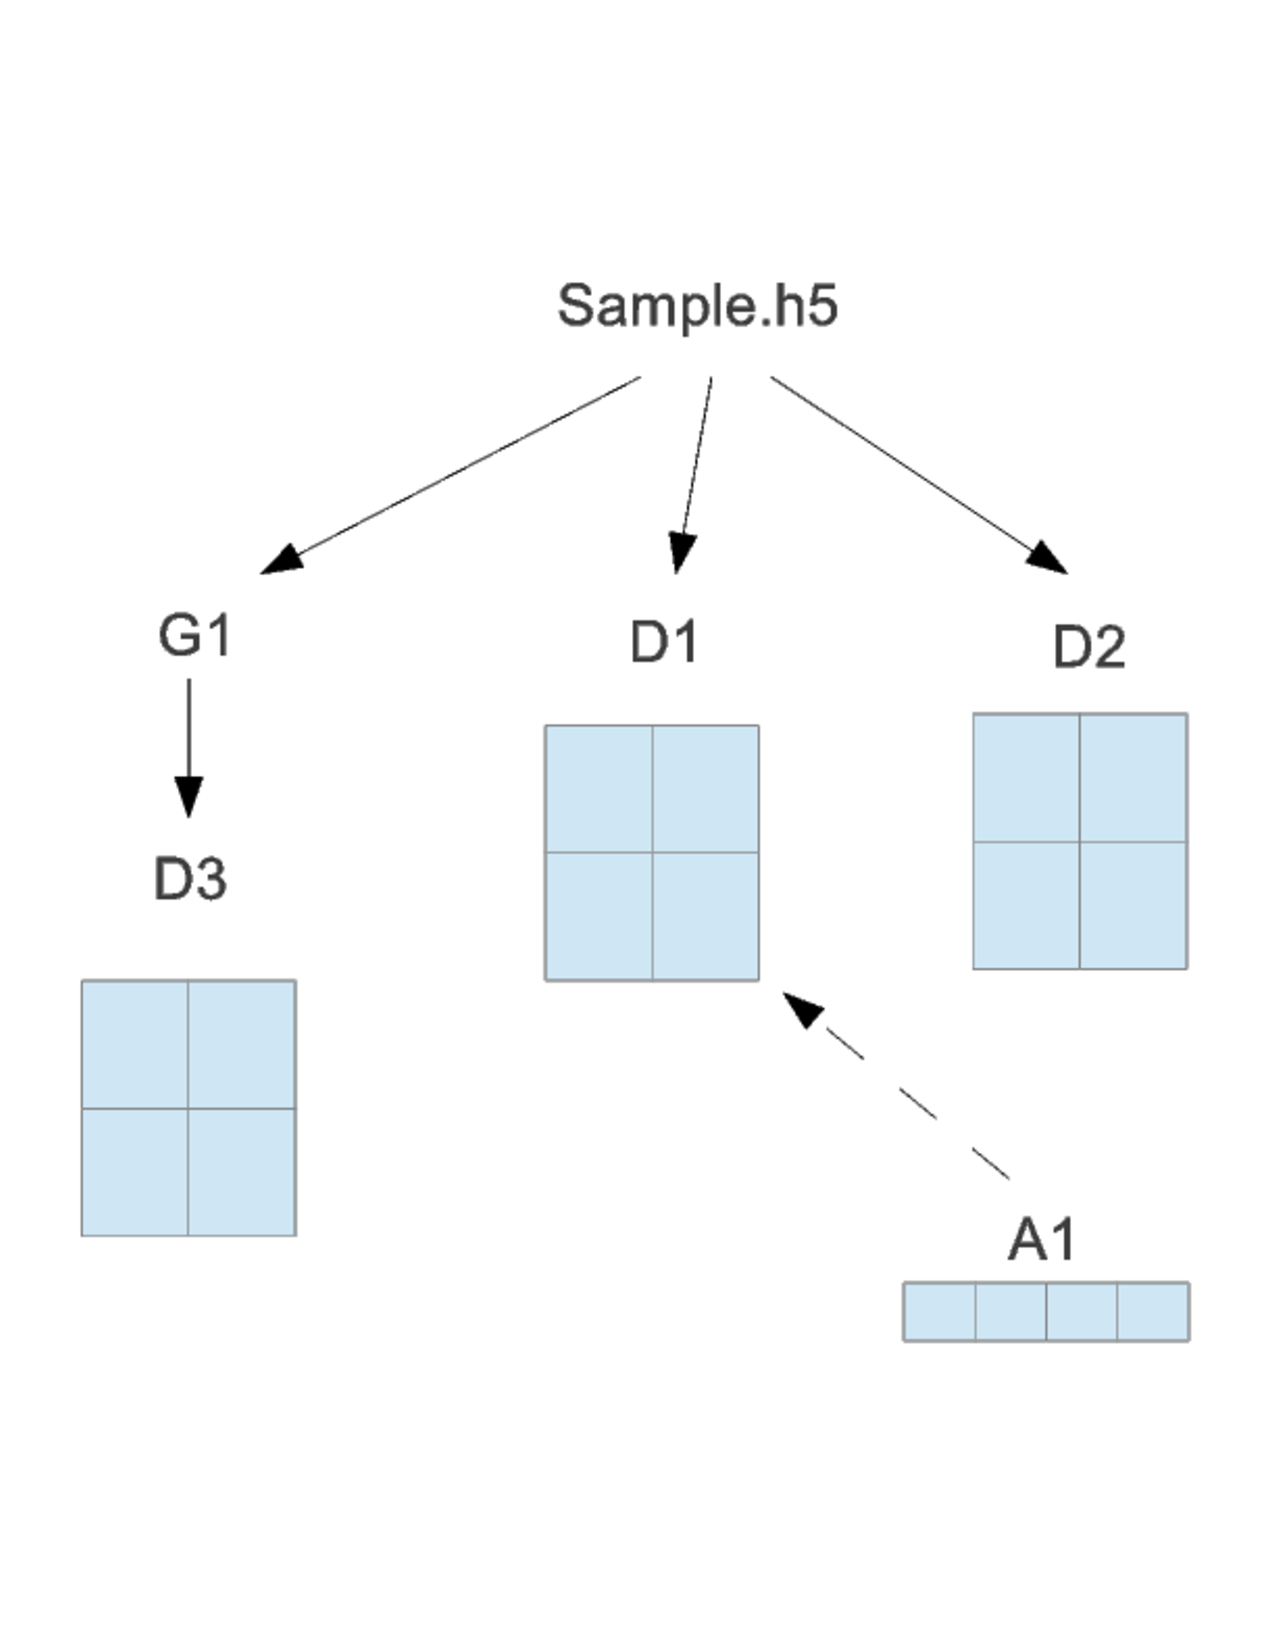
\includegraphics[width=2.5in]{hdf5_example}
\caption{A sample HDF5 file}
\label{hdf5_example}
\end{figure}

%Parallel HDF5 (PHDF5):
%HDF5 supports parallelism using MPI. Multiple processes can be used to access objects in a file. PHDF5 exports a parallel I/O interface, internally making use of MPI-IO. 
%Applications typically store multiple objects in a single HDF5 file. However, many popularly used parallel file systems like Lustre, Panasas etc. are known to perform poorly for workloads where multiple processes access a shared file. 

Virtual Object Layer (VOL):
VOL is a new abstraction layer internal to the HDF5 library~\cite{vol}. As shown in figure~\ref{hdf5_vol} it is implemented just below the public API. The VOL exports an interface that allows writing plugins for HDF5, thereby enabling developers to store objects in a format different from the default HDF5 file format (like native netCDF or HDF4 format). Plugin writers provide an implementation for a set of functions that access data on disk. These include functions for file management, dataset creation and access, group creation, to name a few.

\begin{figure}[!t]
\centering
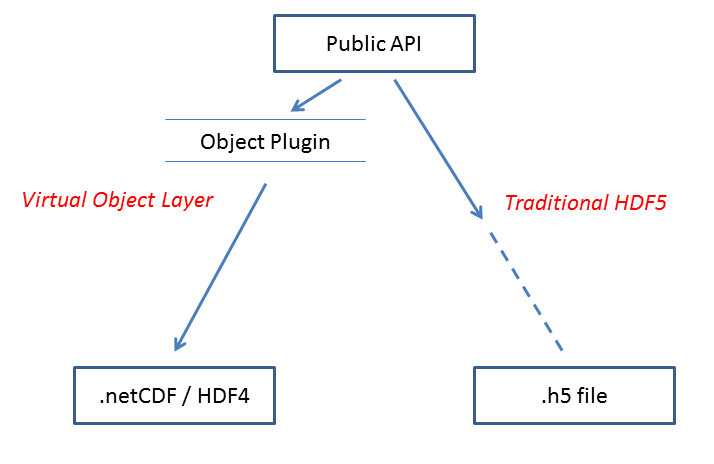
\includegraphics[width=3.5in,height=2.8in]{hdf5_vol}
\caption{Virtual Object Layer (VOL)}
\label{hdf5_vol}
\end{figure}

%\subsection{PLFS}
PLFS is a middleware virtual file system that converts writes to a shared logical file into writes to multiple physical files. 
It is situated between the application and the parallel file system responsible for the actual data storage. 
It transforms N-1 into N-N, where every process participating in I/O writes data to its own, separate file. 
The basic operation of PLFS is as follows. For every writer to a logical file, PLFS creates a unique physical file on the underlying parallel file system. 
It also maintains sufficient metadata to recreate the shared logical file. 
We added a new feature to PLFS called extendible attributes (Xattrs). Xattrs serve as short, extensible metadata stored as key-value pairs.
They can be used to store user-defined information about data for easy and fast retrieval. 
%We use xattrs to store metadata about HDF5 datasets. For example, the datatype, number of dimensions and their extent are stored as xattrs. 

Users can interface with PLFS directly by using the PLFS API or by using its MPI-IO driver (ad\_plfs).  

As stated before, when multiple processes access a single, shared file, file systems like Lustre are known to exhibit sub-standard I/O performance. PLFS has demonstrated benefits of converting this N-1 access pattern into one where every process writes data to its own physical file and sufficient metadata is maintained to recreate the original file in the correct order of writes issued. 
Secondly, the data model of HDF5 stores multiple datasets in a single file on disk. As a result, one cannot perform any useful post-processing on individual HDF5 objects. As we shall see, storing objects in a different file format allows us to perform optimizations on individual HDF5 objects without affecting the remaining data in the file.


\section{Plugin}
We have developed a plugin which stores data in a format which enables performing semantic analysis on the data and uses PLFS for high I/O throughput. 
Instead of storing all objects in a single file, it stores every HDF5 object in a separate location, so that data from different objects is not contained in the same file. In short, we provide a raw mapping of HDF5 objects to the file system. 
HDF5 files and groups are stored as directories, whereas datasets and attributes, which contain raw data, are stored in files created using PLFS. 
Consider the example shown in figure~\ref{hdf5_example}. Using the plugin, file Sample.h5 is stored as a directory. Group G1 is stored as a directory under it, and datasets D1 and D2 are files. Attribute A1 is a file created at the same location as dataset D1 to which it is attached. Additionally, the name of the attribute is stored as \textit{dataset name}.\textit{attribute name} to denote the dataset to which the attribute is attached. Thus these objects are stored at the following paths:\\
/Sample.h5/\\
/Sample.h5/G1\\
/Sample.h5/G1/D3\\
/Sample.h5/D1\\
/Sample.h5/D1.A1\\
/Sample.h5/D2\\

We can see that the relationship between the objects is represented by their relative paths at the file system. That is, the path /Sample.h5/G1/D3 tells us that D3 is a dataset belonging to Group G1 under the root group of the file. This approach gives us the ability to distinguish HDF5 objects inside the storage system. Also, the plugin eliminates the need to explicitly store the metadata describing the relationship between objects. Metadata about datasets, such as the datatype, extent, dimensions etc. are stored as Xattrs. 
 
%\begin{figure}[!t]
%\centering
%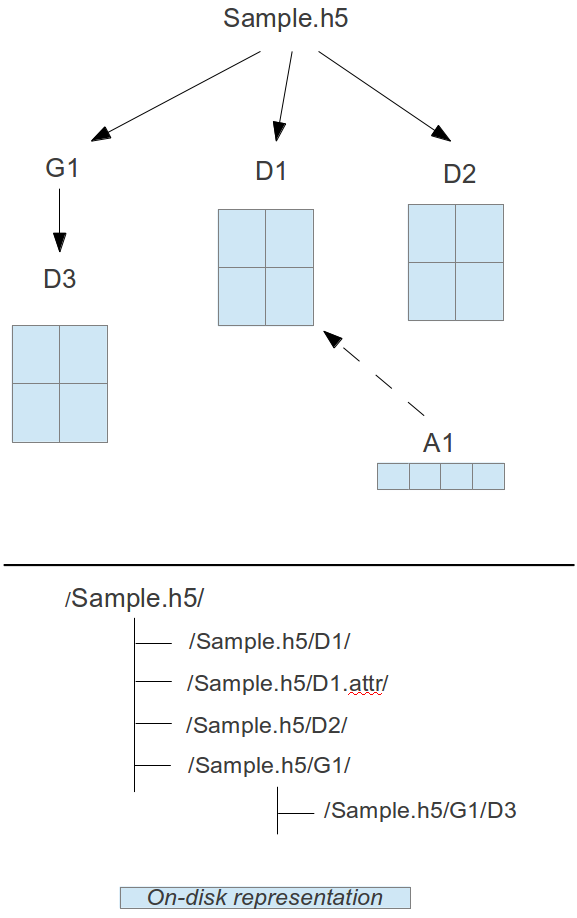
\includegraphics[width=2.5in]{hdf5_example_plugin}
%\caption{HDF5 file created using our PLFS plugin}
%\label{hdf5_example_plugin}
%\end{figure}


Our plugin makes direct calls to the PLFS API. For the current version, we do not support collective I/O operations. It should be noted that HDF5 when used natively with MPI-IO allows users to specify whether collective I/O should be used for reading and writing data. 

The above format of storing data allows us to perform at least two different analysis optimizations.  To illustrate via an example, imagine storing a three-dimensional ocean model within a PLFS file. The storage system sees the file as an opaque linear array of bytes.  With the structure, however, PLFS can provide \textit{active analysis} as well as \textit{semantic restructuring}.  

Active analysis borrows the transducers idea from the Semantic File System~\cite{semantic_fs} which has since been productized in Google's BigTable and Apache Hbase technologies~\cite{google_coprocessors,GFS,apache_hbase}.  With active analysis, the application can ship a data parser function when it creates the PLFS file.  As the data is written into PLFS, PLFS can apply the data function on the streaming data.  The function will output key-value pairs which PLFS can embed in its extensible metadata.  In this example, one simple function might record the height of the largest wave.  Due to PLFS's model of storing a logical file across multiple physical files, the PLFS extensible metadata can record the height of the largest wave within each physical file.  However, given that PLFS now understands the structure of the logical file, these multiple physical files, within the PLFS container, are more accurately thought of as shards.  In a future burst buffer architecture~\cite{burst_buffers}, these semantic shards will be spread across multiple burst buffer nodes.  Therefore, subsequent analysis of the ocean model can quickly find the burst buffer containing the shard with the largest wave by searching a small amount of extensible metadata instead of scanning the entire ocean model.

Semantic restructuring is the idea of reorganizing the data into a new set of semantic shards.  This would be done to speed future analysis routines.  For example, assume that the ocean model was originally sharded using a row-order organization (i.e. across latitude instead of longitude).  An analysis routine which will explore the model along a column-ordering will suffer poor performance with the row-order organization as its access pattern will result in a large number of small reads from a large set of semantic shards.  However, by knowing the semantic structure, the analysis routine can request a semantic restructuring which will be a compact, intuitively described request such as "restructure into row-ordering."  Without structural knowledge, a semantic restructuring would be significantly more complicated: the analysis routine would have to send a large list of logical offsets to PLFS to inform it of expected read patterns.  In an exascale system, the list of logical offsets will be in the order of one billion.  Semantic restructuring shrinks the size of the request to a small constant value.

%The following table lists the VOL functions currently provided by the PLFS plugin:
%\begin{itemize}
%\item Attribute yes
%\item Dataset yes
%\item File yes
%\item Group yes
%\item Object No
%\item Link No
%\end{itemize}


\section{Evaluation}
For evaluation purposes, we have used HDF5's \textit{h5perf} performance tool~\cite{h5perf}. It allows configuring various parameters, such as the number of processes to run the test with, number of datasets to be created in the file, amount of data contributed by each process per dataset, amount of data read/written by a process in a single I/O call (transfer size) etc. For our measurements, we created 10 datasets in the file, and the total file size was 64 GB or more.

All tests were performed on the Lustre parallel file system~\cite{lustre} on the Atlas cluster at University of Dresden. The file system has 12 OSTs with a stripe size of 1MB. The file system is connected to the compute nodes using an SDR Infiniband link. It should be noted that the file system is in production and subject to demanding and varying workload. We present here the average bandwidth values of 3 runs, though in certain cases, we have seen significant variation.
The cluster has 92 AMD Opteron nodes with 64 cores each and 64 to 512 GB memory. 

We have performed tests with 1,2,4,8,32 and 64 processes. We spawned a maximum of 4 processes per node.
Reads and writes are either contiguous or interleaved; processes either access contiguous locations in file or execute a strided pattern.
We compare the performance of the default MPI-IO driver, our plugin, and the PLFS MPI-IO driver (ad\_plfs). 

In Figure~\ref{write_contig}, we show the write performance for a transfer size of 1MB for contiguous writes, for varying number of processes. It can be seen that the plugin regularly outperforms MPI-IO. However, as we increase the number of processes, its performance falls below that of ad\_plfs. Figure~\ref{read_contig} shows the performance of contigous reads for an unaligned transfer size. The plugin again outperforms MPI-IO, but the performance of ad\_plfs is the best for 64 processes. 
%Figure~\ref{write_interleaved} shows the performance of unaligned writes for a maximum of 8 processes. We set the transfer size here to be 10 bytes more than 1MB. Also, the writes here are interleaved as opposed to contiguous. We see a similar pattern, where the plugin outperforms MPI-IO, but is not as good as that of ad\_plfs for 8 processes. 
Figure~\ref{write_collective} compares the performance of MPI-IO with that of the plugin for collective, unaligned, interleaved writes for a maximum of 8 processes. It is important to note that the plugin outperforms MPI-IO in collective mode. We have not been able to obtain results for collective ad\_plfs due to resource restrictions.   

Overall, our results show that although the plugin generally shows good performance, it does not scale as well as we increase the number of processes. This is due to the fact that since we are directly making calls to the PLFS API, the metadata overhead seems to be high. We have all processes participating in file open and close operations, which for large problem sizes can add siginificant overhead. Hence, for future work, we plan to use ad\_plfs directly in the plugin which can overcome this performance drawback, since ad\_plfs has collective optimizations in open and close. It should however be noted that there are some MPI libraries tailored to suit a specific purpose and which do not provide an implementation for MPI-IO. Such libraries can benefit from using a plugin that does not rely on MPI-IO. 

\begin{figure}[!t]
\centering
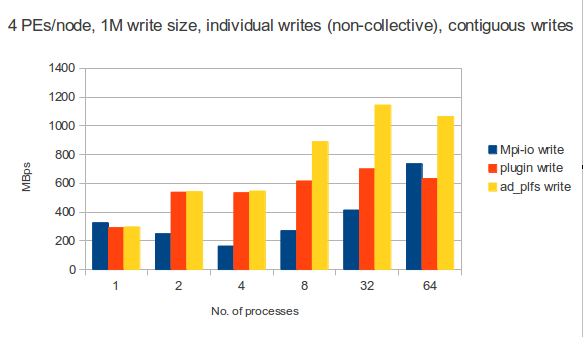
\includegraphics[width=2.5in]{4PEs_node_1M_contig_ind_writes}
\caption{Performance of contiguous writes}
\label{write_contig}
\end{figure}

\begin{figure}[!t]
\centering
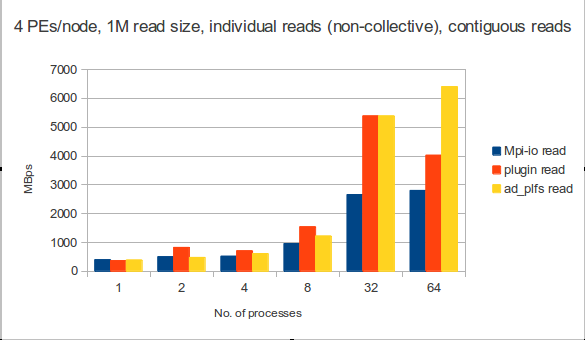
\includegraphics[width=2.5in]{4pes_node_1m_ind_read}
\caption{Performance of contiguous reads}
\label{read_contig}
\end{figure}

%\begin{figure}[!t]
%\centering
%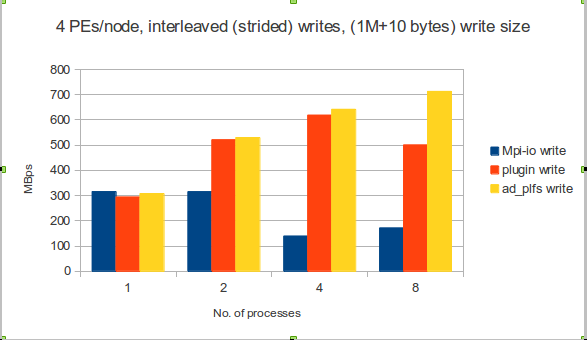
\includegraphics[width=2.5in]{interleaved_1M10_4pes_writes_noncoll}
%\caption{Performance of interleaved writes}
%\label{write_interleaved}
%\end{figure}

\begin{figure}[!t]
\centering
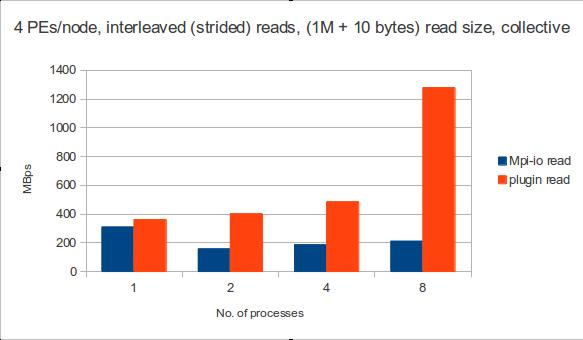
\includegraphics[width=2.5in]{4pes_interleaved_1m10_coll_reads}
\caption{Performance of collective writes}
\label{write_collective}
\end{figure}



% Computer Society journal papers do something a tad strange with the very
% first section heading (almost always called "Introduction"). They place it
% ABOVE the main text! IEEEtran.cls currently does not do this for you.
% However, You can achieve this effect by making LaTeX jump through some
% hoops via something like:
%
%\ifCLASSOPTIONcompsoc
%  \noindent\raisebox{2\baselineskip}[0pt][0pt]%
%  {\parbox{\columnwidth}{\section{Introduction}\label{sec:introduction}%
%  \global\everypar=\everypar}}%
%  \vspace{-1\baselineskip}\vspace{-\parskip}\par
%\else
%  \section{Introduction}\label{sec:introduction}\par
%\fi
%
% Admittedly, this is a hack and may well be fragile, but seems to do the
% trick for me. Note the need to keep any \label that may be used right
% after \section in the above as the hack puts \section within a raised box.



% The very first letter is a 2 line initial drop letter followed
% by the rest of the first word in caps (small caps for compsoc).
% 
% form to use if the first word consists of a single letter:
% \IEEEPARstart{A}{demo} file is ....
% 
% form to use if you need the single drop letter followed by
% normal text (unknown if ever used by IEEE):
% \IEEEPARstart{A}{}demo file is ....
% 
% Some journals put the first two words in caps:
% \IEEEPARstart{T}{his demo} file is ....
% 
% Here we have the typical use of a "T" for an initial drop letter
% and "HIS" in caps to complete the first word.
%\IEEEPARstart{T}{his} demo file is intended to serve as a ``starter file''
%for IEEE Computer Society journal papers produced under \LaTeX\ using
%IEEEtran.cls version 1.7 and later.
% You must have at least 2 lines in the paragraph with the drop letter
% (should never be an issue)
%I wish you the best of success.

%\hfill mds
 
%\hfill January 11, 2007

%\subsection{Subsection Heading Here}
%Subsection text here.

% needed in second column of first page if using \IEEEpubid
%\IEEEpubidadjcol

%\subsubsection{Subsubsection Heading Here}
%Subsubsection text here.


% An example of a floating figure using the graphicx package.
% Note that \label must occur AFTER (or within) \caption.
% For figures, \caption should occur after the \includegraphics.
% Note that IEEEtran v1.7 and later has special internal code that
% is designed to preserve the operation of \label within \caption
% even when the captionsoff option is in effect. However, because
% of issues like this, it may be the safest practice to put all your
% \label just after \caption rather than within \caption{}.
%
% Reminder: the "draftcls" or "draftclsnofoot", not "draft", class
% option should be used if it is desired that the figures are to be
% displayed while in draft mode.
%
%\begin{figure}[!t]
%\centering
%\includegraphics[width=2.5in]{myfigure}
% where an .eps filename suffix will be assumed under latex, 
% and a .pdf suffix will be assumed for pdflatex; or what has been declared
% via \DeclareGraphicsExtensions.
%\caption{Simulation Results}
%\label{fig_sim}
%\end{figure}

% Note that IEEE typically puts floats only at the top, even when this
% results in a large percentage of a column being occupied by floats.
% However, the Computer Society has been known to put floats at the bottom.


% An example of a double column floating figure using two subfigures.
% (The subfig.sty package must be loaded for this to work.)
% The subfigure \label commands are set within each subfloat command, the
% \label for the overall figure must come after \caption.
% \hfil must be used as a separator to get equal spacing.
% The subfigure.sty package works much the same way, except \subfigure is
% used instead of \subfloat.
%
%\begin{figure*}[!t]
%\centerline{\subfloat[Case I]\includegraphics[width=2.5in]{subfigcase1}%
%\label{fig_first_case}}
%\hfil
%\subfloat[Case II]{\includegraphics[width=2.5in]{subfigcase2}%
%\label{fig_second_case}}}
%\caption{Simulation results}
%\label{fig_sim}
%\end{figure*}
%
% Note that often IEEE papers with subfigures do not employ subfigure
% captions (using the optional argument to \subfloat), but instead will
% reference/describe all of them (a), (b), etc., within the main caption.


% An example of a floating table. Note that, for IEEE style tables, the 
% \caption command should come BEFORE the table. Table text will default to
% \footnotesize as IEEE normally uses this smaller font for tables.
% The \label must come after \caption as always.
%
%\begin{table}[!t]
%% increase table row spacing, adjust to taste
%\renewcommand{\arraystretch}{1.3}
% if using array.sty, it might be a good idea to tweak the value of
% \extrarowheight as needed to properly center the text within the cells
%\caption{An Example of a Table}
%\label{table_example}
%\centering
%% Some packages, such as MDW tools, offer better commands for making tables
%% than the plain LaTeX2e tabular which is used here.
%\begin{tabular}{|c||c|}
%\hline
%One & Two\\
%\hline
%Three & Four\\
%\hline
%\end{tabular}
%\end{table}


% Note that IEEE does not put floats in the very first column - or typically
% anywhere on the first page for that matter. Also, in-text middle ("here")
% positioning is not used. Most IEEE journals use top floats exclusively.
% However, Computer Society journals sometimes do use bottom floats - bear
% this in mind when choosing appropriate optional arguments for the
% figure/table environments.
% Note that, LaTeX2e, unlike IEEE journals, places footnotes above bottom
% floats. This can be corrected via the \fnbelowfloat command of the
% stfloats package.



\section{Conclusion}
Using HDF5's virtual object layer, we have developed a new plugin that makes use of PLFS for improved I/O performance. We deviate from HDF5's native file format and store data in a way that allows us to perform useful post-processing on individual HDF5 objects. 
Such a format can further allow us to incorporate semantic analysis of data for burst buffer type workloads. 
Initial results show that our plugin outperforms MPI-IO in most cases, whereas MPI-IO when used with PLFS's MPI-IO driver shows the best results. 


%The conclusion goes here.





% if have a single appendix:
%\appendix[Proof of the Zonklar Equations]
% or
%\appendix  % for no appendix heading
% do not use \section anymore after \appendix, only \section*
% is possibly needed

% use appendices with more than one appendix
% then use \section to start each appendix
% you must declare a \section before using any
% \subsection or using \label (\appendices by itself
% starts a section numbered zero.)
%


\appendices
%\section{Proof of the First Zonklar Equation}
%Appendix one text goes here.

% you can choose not to have a title for an appendix
% if you want by leaving the argument blank
%\section{}
%Appendix two text goes here.


% use section* for acknowledgement
%\ifCLASSOPTIONcompsoc
  % The Computer Society usually uses the plural form
  \section*{Acknowledgments}
  We would like to thank Mohamad Chaarawi and Quincey Koziol from the HDF group for their help with the development of the plugin. We would also like to thank University of Dresden, Germany for the use of their Atlas cluster hosting the Lustre file system.


%\else
  % regular IEEE prefers the singular form
 % \section*{Acknowledgment}
%\fi


%The authors would like to thank...


% Can use something like this to put references on a page
% by themselves when using endfloat and the captionsoff option.
\ifCLASSOPTIONcaptionsoff
  \newpage
\fi



% trigger a \newpage just before the given reference
% number - used to balance the columns on the last page
% adjust value as needed - may need to be readjusted if
% the document is modified later
%\IEEEtriggeratref{8}
% The "triggered" command can be changed if desired:
%\IEEEtriggercmd{\enlargethispage{-5in}}

% references section

% can use a bibliography generated by BibTeX as a .bbl file
% BibTeX documentation can be easily obtained at:
% http://www.ctan.org/tex-archive/biblio/bibtex/contrib/doc/
% The IEEEtran BibTeX style support page is at:
% http://www.michaelshell.org/tex/ieeetran/bibtex/
{\scriptsize
%\bibliographystyle{IEEEtran}
\bibliographystyle{plain}
% argument is your BibTeX string definitions and bibliography database(s)
%\bibliography{IEEEabrv,paper}
\bibliography{paper}
}
%
% <OR> manually copy in the resultant .bbl file
% set second argument of \begin to the number of references
% (used to reserve space for the reference number labels box)
%\begin{thebibliography}{1}

%\bibitem{IEEEhowto:kopka}
%H.~Kopka and P.~W. Daly, \emph{A Guide to {\LaTeX}}, 3rd~ed.\hskip 1em plus
%  0.5em minus 0.4em\relax Harlow, England: Addison-Wesley, 1999.

%\end{thebibliography}

% biography section
% 
% If you have an EPS/PDF photo (graphicx package needed) extra braces are
% needed around the contents of the optional argument to biography to prevent
% the LaTeX parser from getting confused when it sees the complicated
% \includegraphics command within an optional argument. (You could create
% your own custom macro containing the \includegraphics command to make things
% simpler here.)
%\begin{biography}[{\includegraphics[width=1in,height=1.25in,clip,keepaspectratio]{mshell}}]{Michael Shell}
% or if you just want to reserve a space for a photo:

%\begin{IEEEbiography}{Michael Shell}
%Biography text here.
%\end{IEEEbiography}

% if you will not have a photo at all:
%\begin{IEEEbiographynophoto}{John Doe}
%Biography text here.
%\end{IEEEbiographynophoto}

% insert where needed to balance the two columns on the last page with
% biographies
%\newpage

%\begin{IEEEbiographynophoto}{Jane Doe}
%Biography text here.
%\end{IEEEbiographynophoto}

% You can push biographies down or up by placing
% a \vfill before or after them. The appropriate
% use of \vfill depends on what kind of text is
% on the last page and whether or not the columns
% are being equalized.

%\vfill

% Can be used to pull up biographies so that the bottom of the last one
% is flush with the other column.
%\enlargethispage{-5in}



% that's all folks
\end{document}


